
% thesis.tex (also saved as simple.tex) -- a simple thesis document
% for demonstrating dalthesis.cls class file, or to use as a starting
% document for writing a thesis.
% If you are not familiar with TeX and LaTeX, the first thing that you
% can learn that line comments start with the percent sign (%), so
% these lines are ignored by the system.  Feel free to change them or
% delete them.
\documentclass[12pt]{report}
\newcommand{\mychapter}[2]{
    \setcounter{chapter}{#1}
    \setcounter{section}{0}
    \chapter*{#2}
    \addcontentsline{toc}{chapter}{#2}
    }
\usepackage[utf8]{inputenc}
\usepackage{graphicx}
\usepackage{gensymb}
\usepackage{comment}
\usepackage{amsmath}
\usepackage{caption}
\usepackage{subcaption}
\usepackage{pdfpages}
\usepackage[toc,page]{appendix}
\usepackage{afterpage}


% BIB ---------


% BIB ---------

\newcommand\blankpage{%
    \null
    \thispagestyle{empty}%
    \addtocounter{page}{0}%
    \newpage}
\usepackage{hyperref}

\pagenumbering{roman}

\begin{document}


\begin{figure}
 \centering 
 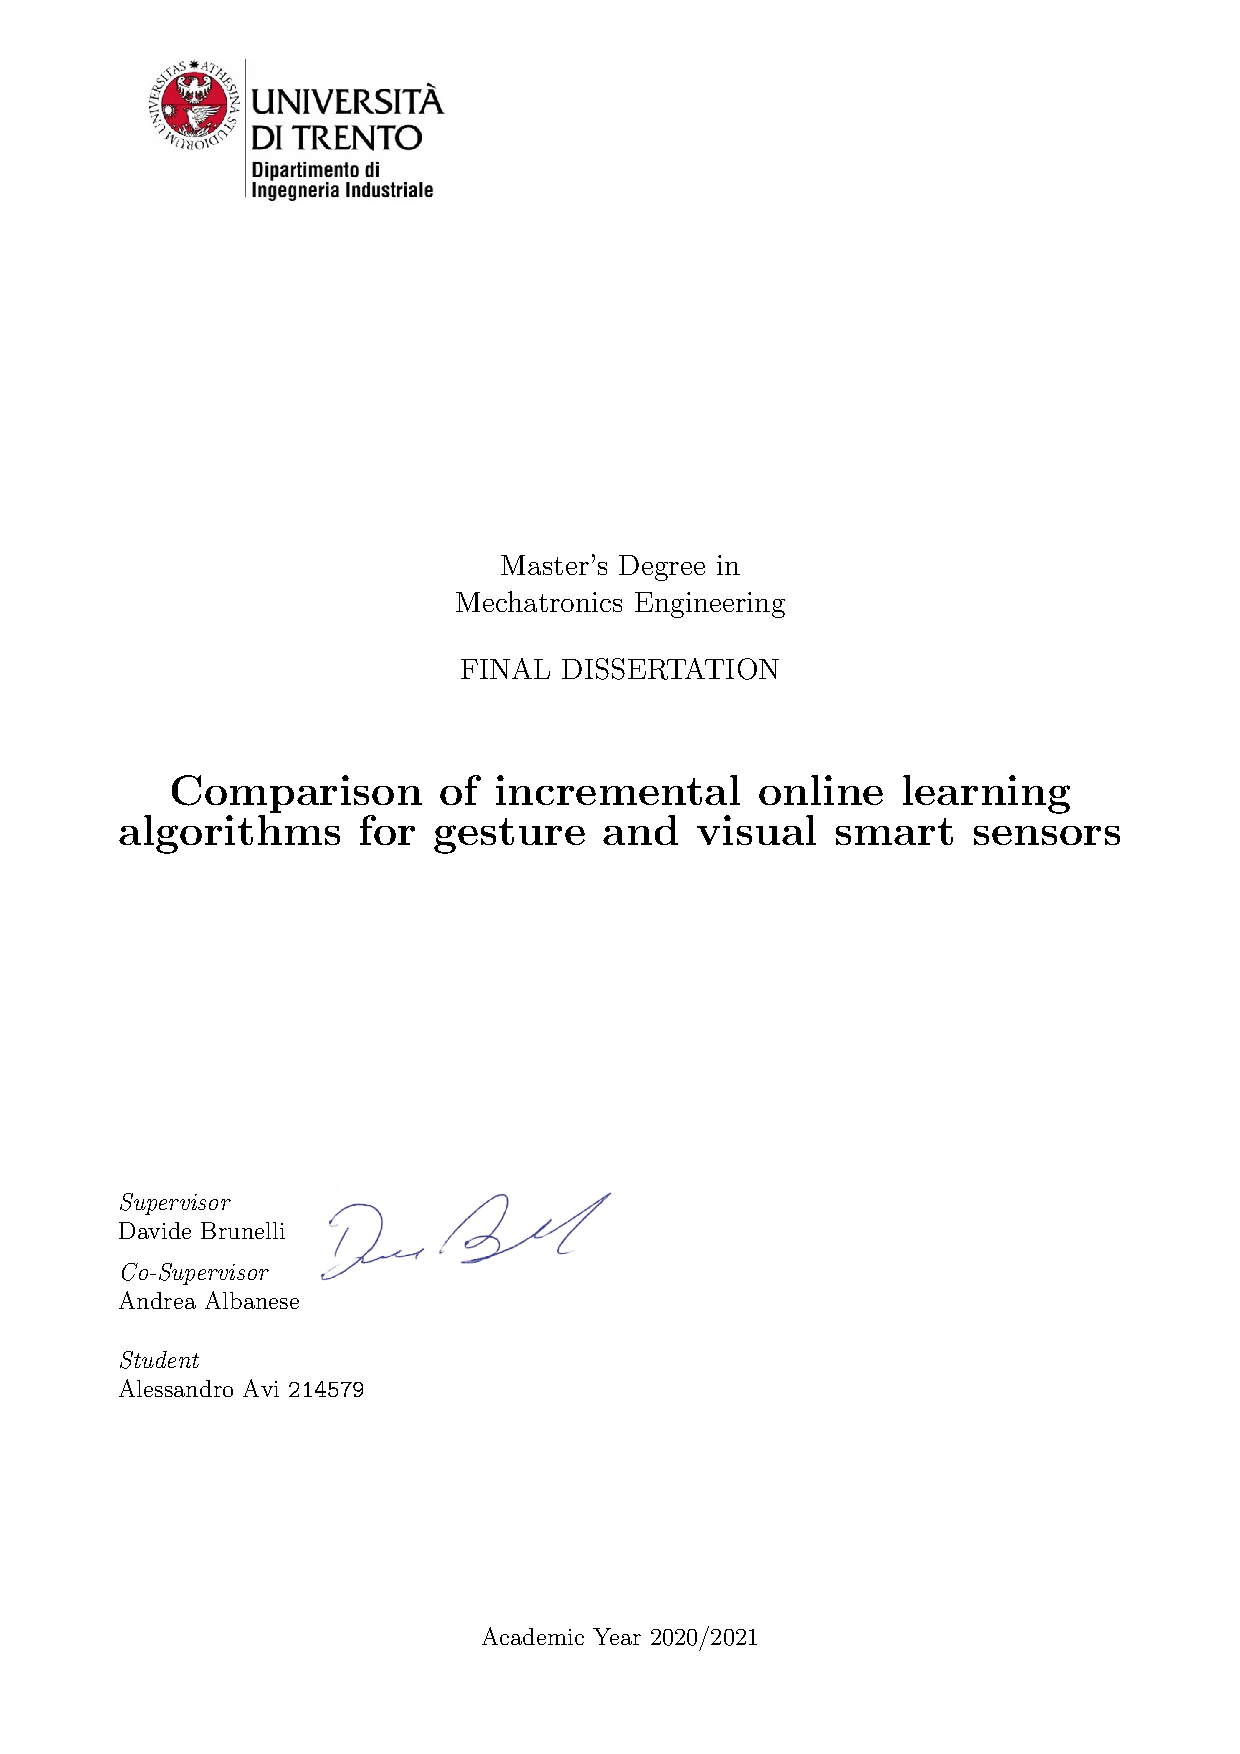
\includepdf[pages=-]{Figures/frontespizio_firmato.pdf}
\end{figure}

\afterpage{\blankpage}

\chapter*{}
\vspace*{\fill}
\textit{"Ciao."} 
\begin{flushright}
Mario
\end{flushright}
\vspace*{\fill}

\afterpage{\blankpage}





%\afterpage{\blankpage}
\tableofcontents
%\afterpage{\blankpage}
\listoffigures
\listoftables
\afterpage{\blankpage}



%\mainmatter

\mychapter{0}{Introduction}
\pagenumbering{arabic}

The application of machine learning (ML) on small devices, in a word TinyML, is becoming more and more popular as technologies advances. The usage of this type of technology on micro controllers (MCU) is proving to be more indispensable and helpful in several fields like the industrial applications, agricultural automation, autonomous driving, human-machine interaction. One of the main fields in which TinyML shines and is well suited is the world of Internet of Things (IoT). Here machine learning applied on small devices finds its sweet spot since it can be exploited to revolutionize the basics of IoT networks. The ability of embedded systems to perform high level and smart data elaboration makes it possible for the IoT pipeline to change from cloud computing to edge computing. This transformation comes with great benefits and additional challenges. 
First of all the traffic on IoT networks is drastically reduced. In fact by performing inferences and predictions directly on the edge the raw data gets compressed into smaller sequences that are enriched of information, reducing the quantity of data moving int the IoT networks. This allows to reduce the energy consumption dedicated to the entire system. In fact by redirecting the energy flow from data transmission to ML computation it's possible to decrease the consumption by and order of magnitude \cite{} SERVE UNA REFERENCE. 
Not only edge computing lowers the traffic but also it reduces the computational weight given to the central point of the entire network, the cloud. This results in reduced times of computation and communication between edge and cloud, which if combined with the ability of the MCU to perform autonomous decision, reduces the latency of real time applications improving the overall experience. 
Another benefit is the improved privacy of the network which is a direct consequence of the reduction of data transmitted. Of course by having less data transmitted also the possibility to have unwanted interceptions is reduced. At last the usage of ML on small devices allows for better customization of the device itself, which can make the devices better suited for the job. 
Of course the application of such a technology comes with a cost, in this case increased complexity and higher amount of vulnerabilities. It's in fact necessary to set up robust systems that are able to ensure the security of the system (due to the high number of vulnerable nodes) and perform at their best, no matter the limitation of the device. It's known that the main downsides of embedded systems and small MCUs are their limited hardware, mainly small memories and batteries. Still these devices are required to perform at their best even with limited computational power and limited power consumption.\\
Another relevant challenge for the application of ML in the world of IoT comes directly from the environment in which these are deployed. Depending on the specific application it's usually the case that the context in which an IoT device lives is not characterized by static behaviour. Meaning that the phenomenon to be monitored is able to change or evolve over time and so does the data recorded. This can make difficult the usage of the ML models because they lack the ability to adapt to the changing scenarios. In fact typical TinyML applications aim at training the models on powerful devices and later deploy them on the MCU, where only the inference is performed. It's clear how these devices are vulnerable to the context change before mentioned. In today's research three different types of scenarios can be defined: New Instances (NI), when new patterns of already known classes are detected; New Classes (NC), when new families of data are found that are not recognized by the system ; New Instances and Classes (NIC), when the data is composed of both new patterns and new classes.
By training ML models for a specific context and later deploying them in the real world is to be expected a drop in prediction accuracy which would make the application itself non reliable. It's then clear how an application of simple ML on such problems is not the best solution. In order to contrast the issue it's necessary to implement what is called Continual Learning (CL). A machine learning approach that allows ML models to be continually kept up to date
This type of machine learning method uses a real time training based on the data incoming, thus allowing the model itself to change and adapt its weights to better contrast the context drift. An additional feature that can be easily added to CL is the recognition of new and never seen classes, that allows the model to also extend its structure in order to better perform inference on the data and be able to recognize new classes. \\
The implementation of CL in industrial applications is not a new topic in the research world, but its implementation on tiny devices is just starting to become more and more popular. The most common applications see CL in industrial scenarios, mainly for monitoring purposes on heavy machines.
The main contributions of this study concern the application of CL in two interesting application. The objective here is to understand if CL is a feasible solution for TinyML and if its usage is actually effective for the generation of autonomous and self adapting models. In this study several state of the art continual learning algorithms are implemented and tested in two experiments, both concerning the application of ML classification on different types of data. The first application regards the analysis of accelerometer data. In this experiment the user holds the accelerometer sensor in its hand and records a time series of accelerations while drawing letters in the air. The idea is to be able to apply ML in order to classify the input data are recognize the letters written. The model created is initially trained for the recognition of the pattern from the vowels. Later CL is applied to the experiment and the model is exposed to new data representing three new consonants. The aim of the experiment is to let the ML model learn the new patterns by performing a real time training. Even if the experiment proposed is closer to an academic study than a real application it's considered to be a clear example of how a CL model could behave in a similar scenario. A popular application of CL in the research is in fact the monitoring of vibration patterns of heavy industrial machinery. The second application sees the experimentation of CL on a CNN model applied on an OpenMV camera for the recognition of the digits from the MNIST dataset. The idea this time is to initially train the model to recognize only the digits from 0 to 5 and later use the CL framework developed for applying a real time training on the remaining digits. This second experiment could be closer to an application, once again in the industry field, where a camera is used for visual control of defects on products in a production pipeline.  \\
The work done for this study is a good example for showing the capabilities of these tiny devices. It proves that machine learning applied on MCUs is a technology that has huge potential and deserves more attention. It could lead to smarter, more efficient, better performing systems in the fields of IOT and applications in the industrial and agricultural world. 

%accennare catastrophic forgetting



\chapter{Related Works}


\section{Machine learning in general}


\section{Machine Learning on MCU}
% applicazione ml su mcu, risorse limitate, molto importante power comsumption, design del mcu, paralre di possibili applicazioni, paraldre del fatto che si fa solo inference
% parlare del rpuning, binarization, compression del meodello, state of teh art compression MCUNET


TinyML is a fast growing research area that aims at applying ML on limited devices like micro controllers. This technology has found a rapid grow in the last years especially thanks to the potential demonstrated by useful applications. The main fields in which TinyML can be applied are human-computer interactions, industrial applications, ... Fare esempi di paper generici su TinyML

The main challenge of TinyML is for sure the successful application of ML on such resource constrained systems. These are in fact designed to be deployed in difficult to reach places and for running for very long times. This implies that the devices should be battery power or equipped with energy harvesting hardware and their power consumption should be limited and optimized. Other limitations concern the limited computational power, which is directly connected to the CPU frequency and the battery management and the available memory. The latter is a very important topic for TinyML. It's in fact known that the application of ML on any type of device requires the usage of great amounts of memory, it's then a big challenge to be able to deploy these systems with very limited memories.\\
The application of ML on MCUs, mobile devices or in general on the edge of IoT systems it's a great advantage that can bring to some improvmenets. The key advantages are:
\begin{itemize}
\item privacy: by having the data directly processed on the node there is no change of violating the privacy policies since the possibility of interception is totally nulled
\item latency: by elaborating data directly on the edge the work load of processing that should be performed by the cloud is limited and so is the transmission of the data itself. This brings to limited time delays and allows the device to perform decisions in real time, improving the performances of real time applications.
\item energy efficiency: the transmission of huge quantities of data from the edge to the cloud takes a big portion of the energy consumption of an IoT system. Even if the application of NN is energy intensive it is an order of magnitude less, thus an improvement.
\end{itemize}


\section{Continual-on line learning}
% spiegare cosa è ctastrophic forgetting, come mai serve, cosa va a risolvere, quali sono i problemi che iontroduce, 
% parlare di cinme CL è trattato nella research, paralkre dlle tipologie di algoritmi, supervised training, frameworks gia sviluppatim metodi di valutazione?

Until recent times the application of ML on MCUs has always been focused on the creation of intelligent small system that maintain good performance with reasonable consumption, limited time of inference and long lifetimes. A major negative aspect of the TinyML solutions is their focus on the inference of streams of data. Which almost always requires the usage of powerful machines for the training of NN models that are later deployed on the MCU. This results in the creation of a static network which is not able to adapt to the data and adjust to different scenarios. The solution to this problem is the creation of a Continual Learning system. \\
CL systems are a variation of the tipical pipeline of ML. The main focus of CL systems is to be able to continuously update the model in order to adapt its structure and parameters to overcome context drift, be able to recognize appearance of new patterns and to avoid catastrophic forgetting. The latter is a problem that is directly introduced by the nature of the paradigm itself. By having a model that is continuously updated with a feedback loop that is directly dependent on the current erross i'ts clear how it's immediate to update the model in such a way that the old tasks are forgetten for the sake of learning the new ones. This could be seen also as a over fitting of the model on the new tasks and if oc course to be avoided. Different algorithms have different ways for contrasting this phenomenon. \\
In todays literature several CL algoprithms and strategies have been already proposed. A well organized summary is proposed in \cite{lesort2020continual}, where the most relevant methods are briefly classified in 4 categories, originally proposed by \cite{maltoni2019continuous}.
\begin{itemize}
\item Architectural: these algorithms are based on the usage of particular types of structures and architectures. Some common methods are weight-freezing, layer activation or dual-memories-models that try to imitate logn term memory and short term memory.
\item Regularization: this group contains all those approaches that base their ability to retain past memories on the application of particular loss functions. In these loss functions usually a term is added with the aim of performing a feedback that considers both the old knowledge and tries to learn the new data.
\item Rehearsal strategies: in these strategies past informations are periodically revisited by the model. This is done for strengthening the old knowledge and connections. Notice that this methods is not well suited for application on MCUs mainly because of the restricted memories. 
\item Generative Replay: this methods implement similar strategies of the rehearsal. This time the data that is repeated in the models is not actually old data saved in the memory but it's actually data artificially generate by the model itself. 
\end{itemize} 

The type of strategies that better suits an application on MCU are for sure the regularization methods and the architectural methods. Both these groups require little to no extra computation with respect to a simple ML application, thus their strength is intrinsic in the update rules adopted. Some of the most important methods from the state of the art are, LWF, PNN, CWR, EWC, SI. 









\chapter{Hardware} 








\chapter{Machine Learning}
% introduzione la machine learning
% spiegare il funzionamento base, nodi, activation function, layers, 
% CNN, NN fully connected, a cosa servono, quali sono gli obbiettivi specifici
% back propagation, sgd, l rate, batch size
% pruning, quantization

Machine learning is a branch of artificial intelligence (AI) and computer science that focuses on the usage of algorithms and huge quantities of data to generate models that are able to perform regression of grey mox models. 

\section{Basic pipeline of the CL system developed}
% spiegare idea di base del CL in questo caso, training fatto in real time
% spiegare come si ottiene la back propagation, far vedere formule, applicate a softmax
% spiegare il sistema fatto a frozen model + OL layer
% spiegare nel dettaglio i metodi implementati + grafici a blocchi che mostrano come va
Continual learning is the application of real time training on a model with the aim of generating self adjusting systems that are able to learn from the incoming data and modify their properties to adapt changes. As well explianed before continual learning in today's technology finds its best application in IoT edge nodes, where ML is applied on small devices to distribute the computation weight over a large number of devices and reduce the traffic over the network. The main advantage brought by CL or OL is that models are then able to autonomosly update their parameters, ability that improves the easo of use of these devices which can then be ddeployed in environemnt with minimal effort for maintainance. \\
In order to apply such a technology on embedded devices is necessary to develop or use the avilabel software and hardware on the market. For this study the hardware uses are just commercially available MCU that are specifically developed for supporting big quantities of computations. The software used by the microcontrollers on the other hand is only partially developed. In both applications it has been possible to use already developed tools specifically built for inference, which is just one of the steps required for a continual learning application. \\
In this study the main idea was to develop something similar to paper TinyOL. The idea is to attach the OL system to the last layer of the pre trained model in order to enhance just the classification aspect of the ML model. The base functions required by the system are basically two: be able to update the weights of the classification layer each time the model shows an error in the prediction array and be able to enlarge the size of the last layer at will, specifically when new classes are detected that should require a new label. The applications seen here are supervised machine learning trainings. This means that at every training step the griund truth label is known and is provided to the algorithm, which will then use these info to compute the error and back propagate this for updating the layer. In fact the feature that allows the model to recognize new classes is performed simply by checking if the label recieved is inside the pool of already known classes. \\
The basic idea of continual learning consists in being able to continually refresh and update the weights and biases of the layer or layers of interest. This is performed as in standard trainings by computing the error performed by the inference and by propagating this error back in the weights themselves. In orrder to do this it's necessary to know the basic structire of the model wich gives informatiosn about the math used by the nodes. If the entire path of computation from the weight of interest to the final prediction is known then it's possible to back propagate the error to the parameter. In this specific study the idea has always been to use CL in classification problems. By havinsuch a specifica field of application it's possil e to simply the CL ide to a restricted group of models. Since the problems regard only classification and this specifica application want sto update only the lsat layer the problem becomes a simple study of the back propagation over softmx layers and nodes. Let's consider a simple model composed of few layer, and asume that the last layer brings 100 nodes of the hidden layer 2 to just 5 nodes with softmax application function. It's then possible to comnsider everythin that happens before the softmax layer a grey box that simply gives us 100 output values. The simple formula that defines the computation obtained in a softmax layer is:

\begin{equation}
y_i = softmax(\sum ) \quad softmac = gigio
\end{equation}

Then on the output obtained by the softmax layer the loss function is applied. There are lots of different loss functions that could be applied, in this case the models were always trained with a loss function called categorical cross entopy, which has the following definition:

\begin{equation}
categorical cross entropy = gigione
\end{equation}

At this point is necessary to find out how the error performed by the model is affected by each single weight. In order to do so a simple derivation is required, which is done in the following way and birngs to a simple solution:

\begin{equation}
calcolo delle derivate
\end{equation}

Then it's immediate to apply this on the weifht in order to apply an actual training step. The final formula that defines the back proapgation on weights and biases of a softmax layer with the usage of a categorical cross entrioyp loss function is:

\begin{equation}
w = w- l rate
\end{equation}

This is the rule to be followd for the application a basic training step in real time. This is also the same idea explored by TinyOL, which simply applies this rule to an autoencoder model for the recognition of patterns. \\


\section{Algorithms implemented}
In this study not only the basic training strategy has been implemented and tested but also other regularization approaches have been used. As explained in the related work section regularization approaches are strategies that exploit the addition of a loss term to the update. Thanks to this it's possible to have some sort of control over the weight update. In today's research the most efficient and common strategies for CL are Elastic Weight Consolidation (EWC), Synaptic Intelligence (SI), Learn Without Forgetting (LWF) \cite{li2017learning} and in a recent paper also Copy Weight with Reinit (CWR) \cite{lomonaco2017core50}, Copy Weight with Reinit+ (CWR+) \cite{maltoni2019continuous} and AR1 \cite{maltoni2019continuous} have been presented. In this study it has been considered opportune to implement and compare the simpler ones which are LWF and CWR, together with the basic TinyOL and a small variations of them. \\
In the applications for this study all methods are applied in the same OL general block system, which simply is attached to a pre trained model, called frozen model. The frozen model is treated as a grey box which simply performs feature extraction on the input array and provides the last layer with useful elaborated data. The OL training is then applied on the weights of the classification layer following the update rule imposed by the algorithm of choice.

\subsubsection{TinyOL}

The TinyOL method applied on MCU has been initially implemented in paper \cite{ren2021tinyol}. Its implementation is quite easy since it consists in just some for loops applied correctly on the weights and biases. As explained before, this method uses the basic rule of the training step which consists of propagating the error committed at inference to the weight of interest by using SGD. Keep in mind that the activation function of the last layer is Softmax and the loss function is always Categorical Cross Entropy. This said the weights update rule for this algorithm are:
%
\[ \mathcal{L}_{cross}(y_i, t_i)= - \sum_i t_i log(y_i) + (1-t_i)\cdot log(1-y_i)  \]
\[    w_{i,j} = w_{i,j} - \alpha (y_i - t_i) \cdot x_i \]
\[    b_i = b_i - \alpha (y_i - t_i) \]
\[    \text{where i=0,1..,n  and  j=0,1,..,m} \]
%
Where $y_i$ is the prediction obtained from the OL layer, $t_i$ is the true label, $\alpha$ is the learning rate (tuned by the user), $w_{i,j}$ are the weights of the OL layer, $b_i$ are the biases of the OL layer, $n$ is the max amount of classes known by the OL system and $m$ is the height of the last layer of the frozen model. Note that in this entire study the number $n$ can change dynamically since the maximum amount of possible classes is not known a priori, or at least it ism not known in a real life scenario. \\
Also a variation of this method has been implemented. The variation takes into consideration the possibility to use batches of data for computing the back propagation and not simply the last sample received. The idea for implementing such a variation came thanks to the article \cite{batch_size_medium}, where the author explores the impact that batch size has on the training dynamics. The base idea of the variation is that by using a batch of samples bigger than 1 the back propagation computed should not relay on just the last sample but on the average computed on the group. This should help the model to be less vulnerable to noisy data and outliers. In order to apply the algorithm with this variation it's necessary to store the data generated from the previous samples. This requires the allocation of double the amount of memory required for the standard version, which is done with the creation of the matrix W and B. In order to reduce the amount of computation at each training step at first the inference is performed, after this the back propagation for each single weight and bias is computed and its value is added inside the matrices W and B. When the batch finishes the average on each weight and bias is computed and applied on the actual parameter that was kept constant during the entire inference of the batch. This time the update rule at each inference step becomes:
    \[     W_{i,j} = W_{i,j} + \alpha (y_i - t_i) \cdot x_i\]
    \[     B_i = B_i + \alpha  (y_i - t_i) \]
And at the end of every batch the update applied on the real weights is:
    \[     w_{i,j} = w_{i,j} - \frac{1}{batch\_size} \cdot W_{i,j} \] 
    \[     b_i = b_i - \frac{1}{batch\_size} \cdot B_i \]
    
Said this both methods are quite simple and are based on the same basic principle. The method TinyOL requires the usage of only one weight matrix and one bias array. their dimension depend on two parameters, the number of classes known by the OL system represented by the value $n$ and the size of the last layer of the frozen layer, represented by the value $m$. This makes the memory allocated from the method be equal to a total of (nxm+nx1)*4 bytes. The method is able to change the layer parameters each time a new sample is received with no constraints. This feature is the main problem that concerns this strategy. In fact it allows for a lot of flexibility but it doesn't provide a protection from catastrophic forgetting catastrophic forgetting. By allowing any possible modification it's immediate for the model to follow what the stream of data is imposing to it, thus it's quite easy to train on noisy or outliers data or even be guided towards context drift.  \\
On the other hand the method TinyOL with mini batches exploits the same approach seen by the standard TinyOL method but receives a back propagation update that is dictated by the average computed from a group of $k$ samples. Depending on the value of $k$ the group can be considered to be a more or less good representation of the data received. In any case this method should be able to better contrast catastrophic forgetting, noisy data and outliers. 

\subsubsection{TinyOL V2}

The TinyOL V2 algorithms is based on the same idea of the original TinyOL. A little intuible modification is applied in the method with the aim of contrasting catastrophic forgetting. The idea is to remove the possibility to have a drift over the original weights by removing completely this possibility. This algorithm in fact applies the same exact update rule on its parameters but it applies it only on the weights that represent the new classes. Which simply means that the rule now becomes:
    \[ w_{i,j} = w_{i,j} - \alpha (y_i - t_i) \cdot x_i \]
    \[ b_i = b_i - \alpha (y_i - t_i) \]
    \[ \text{where i=p,p+1..,n  and  j=0,1,..,m} \]
The only difference is in fact the iterator $i$, which goes from p to n, where $p$ represents the position of the first unknown class. \\
Also in thsi case the variation of the method for working on batches has been implemented. Again the algorithm is the same as TinyOL with batches but with the iterator $i$ that goes from $p$ to $n$.
    \[     W_{i,j} = W_{i,j} + \alpha (y_i - t_i) \cdot x_i\]
    \[     B_i = B_i + \alpha  (y_i - t_i) \]
And at the end of every batch the update applied on the real weights is:
    \[     w_{i,j} = w_{i,j} - \frac{1}{batch\_size} \cdot W_{i,j} \] 
    \[     b_i = b_i - \frac{1}{batch\_size} \cdot B_i \]
    \[ \text{where i=p,p+1..,n  and  j=0,1,..,m} \]
In conclusion TinyOL V2 is a simple method that differs from the original only because of a small difference in the update rule. By forcing the update on only a portion of the weight and biases the behaviour of the catastrophic forgetting that tries to modify the original knowledge and make the model drift from that context is completely removed. This helps the algorithm by contrasting catastrophic forgetting but also reduces the ability of the model to perform fine tuning on those specific classes. Another negative aspect regards the general behaviour of the final mode. By having a training strategy that updates only a portion of weights it's clear how the model itself cannot be optimized to reduce the loss function. This means that at the end of the training the model will be composed of two parts that will not work together to find the best prediction. Like before the TinyOL V2 with mini batches allows the model to learn from a bigger group of samples, this should help the model to avoid over fitting, outliers and noisy data. \\
The method TinyOL V2 requires the same amount of memory that was used by TinyOL, which means a matrix of size $n \times m$ and an array of size $n \times 1$. On the other hand the method TinyOL V2 with batches requires an additional matrix and array but this time with a reduced size of $(n-p) \times m$ and $(n-p) \times m$ since only the weight of the new classes require an update. 

\subsubsection{LWF}

The LWF strategy is a regularization approach introduced in \cite{li2017learning} and later applied with small variation in \cite{maltoni2019continuous}. The main idea of the method is to contrast catastrophic forgetting by applying a smart loss function and double architecture that is able to combine old and new knowledge in the back propagation of the parameters. The double architecture models refers to the fact that two models are required in order to use this method. In this case the entire OL system has been applied only on the last layer of the model so the double architecture in this case is composed only of a double classification layer. The first is called $tl$, training layer while the second is called $cl$, copy layer. The role of $tl$ is to be continuously updated at each training step with the LWF back propagation rule, while $cl$ is a layer that contains a copy of all the original weights computed in the Tensorflow training, thus it represents the original knowledge of the model. The back propagation rule is based on the idea of fusing the weight updates that the two layer would apply. The fusion of these two updates is done with a weighted average that changes dynamically as the training continues. This of course implies that both layers produce a prediction, which means double computation for the OL system.\\
At this point the only major difference with respect to the TinyOL method is the double inference and the computation of the weighted back propagation. The update to be applied can be computed quite easily again by using SGD which turn out to be a simple weighted sum of two back propagation:
%
\[    \mathcal{L}_{LWF} ( y_i, z_i, t_i) =  (1-\lambda) \cdot{L}_{cross}(y_i, t_i) + \lambda \cdot{L}_{cross}(y_i, z_i) \]
\[ w_{i,j} = w_{i,j} - \alpha \cdot x_i \cdot [ (y_i - t_i)(1-\lambda) + (y_i - z_i)\lambda]  \]
\[ b_i = b_i - \alpha \cdot [ (y_i - t_i)(1-\lambda) + (y_i - z_i)\lambda] \]
\[ \text{where i=0,1..,n  and  j=0,1,..,m } \]
%
Where $y_i$ is the prediction array obtained from the layer $tl$, $z_i$is the prediction array obtained from the layer $cl$, $t_i$ is the ground truth label, $\lambda$ is the variable weight that defines which prediction has more decisional power. \\
The back propagation is composed of two parts, the first defined by $tl$ and the second defined by $cl$. The value $\lambda$ plays a very important role in this update. As explained in \cite{maltoni2019continuous} its value cannot stay constant because it would be suboptimal. In their application the value follows a discrete function linear with the number of batches encountered, while in oiur case its value needed to be dependant on the only value known in a OL application, the amount of samples elaborated. The update of the loss function weight is the following:
\[ \lambda = \frac{100}{100+ \text{prediction$\_$counter}} \]
Another important note to be said is that in the update rule the implementation follows the variation proposed in \cite{maltoni2019continuous}, where the loss functions ${L}_{LWF}$ used in the weighted average are not a balance between categorical cross entropy and knowledge distillation but a balance between two categorical cross entropy. This is a little modification that allows for an easier implementation without ruining the performance. \\
Also in this case a version that integrates batches is proposed. This time the method simply updates the values of $cl$ every time a batch is finished. The  algorithm this time simply becomes a fusion between old and knew knowledge where the old knowledge is refresh once in a while. In this way the model can be seen as a model that performs a weighted average in between a fast learning memory and a memory that stops in time. The size of a batch is defined by the value $k$. 
%
\[    \mathcal{L}_{LWF} ( y_i, z_i, t_i) =  (1-\lambda) \cdot{L}_{cross}(y_i, t_i) + \lambda \cdot{L}_{cross}(y_i, z_i) \]
\[ w^{TL}_{i,j} = w^{TL}_{i,j} - \alpha \cdot x_i \cdot [ (y_i - t_i)(1-\lambda) + (y_i - z_i)\lambda]  \]
\[ b^{TL}_i = b^{TL}_i - \alpha \cdot [ (y_i - t_i)(1-\lambda) + (y_i - z_i)\lambda] \]
\[ \text{where i=0,1..,n  and  j=0,1,..,m } \]
%
And at the end of a batch (once every $k$ values are elaborated):
\[ w^{CL}_{i,j} = w^{TL}_{i,j}  \]
\[ b^{CL}_i = b^{TL}_i  \]
This method, being different from the previous, requires also a different $\lambda$ rule. Experimentally it has been found to be well working an update rule defines as follows:
\begin{equation}
\lambda = \left\{
        		\begin{array}{ll}
            		1                                                         & prediction \_ counter \leq batch \_ size \\
            		\frac{\text{batch$\_$size}}{\text{prediction$\_$counter}} & prediction \_ counter >    batch \_ size
        		\end{array}
    		  \right.
\end{equation}
Both the LWF methods require the same amount of memory, which is a double prediction layer of size  $n \times m$ and $n \times 1$. Both methods are quite easy to implement and their strength is defined in the value $\lambda$ and in their update rule. They differ only from the weight updated applied on the matrix $cl$. A negative aspect that characterizes these two methods is the amount of computation required, which can be a problem for tiny devices. By having two layers and the need of two prediction is of course needed the double of computation. 

\subsubsection{CWR}

CWR is an architectural approach that exploits the usage of two classification layers and a weighted back propagation rule for performing OL. Again the two classification layers are called $tl$, training layer and $cl$, consolidated layer. The idea is to perform training at each step on $tl$ with the same method as TonyOL and at the end of each batch update $cl$ with a particular rule. The back propagations for the $cl$ at the end of a batch are tge same for biases and weights and are the following:
    \[     cw_{i,j} =  \frac{cw_{i,j} \cdot updates_{i} + tl_{i,j}}{updates_{i} + 1} \] 
    \[     tw_{i,j} =  cw_{i,j}\] 
Where $tw_{i,j}$ are the weights and biases of the training layer, $cw_{i,j}$ are the weights and biases of the consolidated layer, and $updates_{i}$ is an array that behaves as a counter of labels encountered.\\
By using two classification layer that update differently the method tries to replicate the short term memory and long term memory architecture that characterizes biological brains ??? ESSERE SICURO. The layer $tl$ behaves as the short term memory since it gets updated at every single training step, and at each batch it gets reset to the correct values. The layer $cl$ behaves as a long term memory since it never gets reset or cleaned and it gets updated only once every batch with a weighted average. This weighting method depends on the number of times that a specific label appeared in the training batch.\\
Another important aspect of this method is how the prediction is computed and used. While performing only training the method requires only a prediction performed by $tl$ since this needs to get updated by its error. However if an actual prediction is requested to the model also the $cl$ layer should perform the computation and provide an inference. In fact the inference obtained by the consolidated layer is to be considered more relevant and reliable since it is produced by the long term memory. In the case a prediction is required the method needs a double prediction, one from $tl$ and the other from $cl$. Again as said for LWF this is not optimal because of the limits of tiny devices. \\
CWR is a method easy to implement. Its strength are hidden in the double architecture and the update rule that make it possible to merge short term memories and long term memories and also contrast catastrophic forgetting. The memory required for this algorithm is: to weight matrices of size $n \times m$, 2 bias arrays of size $n \times 1$, one array that keeps track of the labels encountered of size $n \times 1$. The amount of computations can change depending if a simple training step is performed or if an inference is required.

\subsubsection{AviLearning}




% INSERIRE MODELLO ESEMPIO

And

\section{Pruning and quantization}





\chapter{Experimental set up}

In this chapter the practical aspects of the experiments are explained. Initially the study has been developed entirely on the laptop with Python code with the aim of understanding the theoretical behaviour of the method and the capabilities of CL. Later the same principle and basic pipeline of the framework has been ported to the SMT Nucleo application and to the OpenMV cam. In all applications the idea is to initially train the base model for the recognition of the first few classes. The training is done with Tensorflow and Keras on the laptop and later the model is loaded on the MCU of interest. The CL system which is composed of the OL layer and all the necessary is then attached to work on the output of the frozen model. The idea is to apply different strategies of training only on the last layer in order to be able to perform augmented classifications.  \\
In the next sections all the steps for the correct set up of the entire study are well explained. Starting from the creation and collection of the dataset, then going to the training of the frozen model, implementation of the CL system on the MCUs and finally the actual implementation of the CL system on the devices. 

\section{Dataset collection}

In order to be able to create and train ML models it is necessary to have large quantities of data. In this study the two application explored are applied on two different types of data: time series of accelerometer data and images of hand written digits. \\
The MNIST dataset is a large collection of hand written digits that is publicly available and well known in the academic and research world. It was created in 1998 as a combination of other two smaller databases. Today the dataset is composed of 2 groups of 60000 images for training and 10000 images for testing. The images are gray scaled and have a size of $28 \times 28$ pixels. In today's research world this dataset is used a lot for ML trainings. Its popularity is thanks to its ease of use and its high quality of images which can bring easily to well trained models with high performances.\\
For the purpose of this application the dataset requires some pre processing. Since the goal of the base model is to be able to correctly recognize the digits from 0 to 6 it's necessary to separate the dataset in $low\_digits$ and $high\_digits$. Once this is done two dataset are obtained, the $low\_digits$ dataset contains 36017 samples while the $high\_digits$ dataset contains 23983 samples. After this the separation of the dataset in train, test and validate portions is requested. It has been decided to use the common rule 70-20-10. 
\bigskip
For the accelerometer application the dataset had to be created from zero. To my knowledge there are no publicly available datasets of accelerometer data and in particular no dataset containing examples of hand written letters in the air. The decision that brought to this particular application was simply because of an academic example already seen in class during the lab session of the course of Embedded Systems. In that lab session the aim was the same as this application, classify letters from accelerometer data by applying ML on an MCU. The collection of the dataset has been done with the hardware described in chapter \ref{}, which again is a Nucelo STM32 F401-RE equipped with a Nucleo shield IKS01A2 that mounts a 3D accelerometer sensor. \\
The dataset is composed of 8 different letters, which are A, E, I, O, U, B, R, M. The vowels are the classes that are learned by the base model while the 3 consonants are the letters that are added and learned by the CL system. During the collection of the dataset the MCU is connected via USB to a laptop which has the role of power supplier and live data recorder. In order to collect the data the Nucelo has to run a small script that exploits the usage of some GPIO, timers, interrupts, UART and I2C communication protocols. The idea is that by specifying the letter that is drawn and by pressing the blue button the STM starts to catch data from the accelerometer with the I2C protocol while sending it to the laptop with UART protocol. The data sampling is done at a frequency of 100 Hz and the data stream lasts for 2 seconds, so a total of 200 samples is recorded. Note that a software for serial communication should be used at the same time on the laptop. This is required in order to see in real time the data stream on the laptop and for storing the data somewhere. In this application the software of choice is MobaXTerm which is able to save the entire session communication in a txt file by using the UI. 
Note that a single letter sample is composed of different information. The sample contains the label of the letter drawn, the number of sample saved in the current session and three arrays of 200 values each containing the time series data from the 3 axis of the accelerometer. The final dataset is composed of 5130 samples total, where each vowel counts to an average of xxx samples while the consonants have an average count of 760 samples each. \\
Another important detail is directly connected to the type of context in which the model will be trained and tested. As mentioned in \ref{introduction} the scenarios in which a CL system can live are three, NIC, NC and NI. In order to make the example as close ass possible to real world scenario the dataset was collected keeping in mind a NIC context. This means that the ML model should be exposed to data containing new classes and new patterns of old classes. In order to simulate the new patters of old classes while generating the dataset it has been decided to accentuate some patterns of the hand drawing motion. For example an accentuation of the angles in the letter R, or the velocity at which the letter I is drawn, or the oval shape of the letter O. Keep in mind that all the letters were drawn with the same general motion as shown in Figure[\ref{fig:letters_motion}].\\

\begin{figure}[h!]
    \centering
    
\includegraphics[width=100mm]{Figures/Chapter4/letters_motion.jpg} 
    \caption{Motion of the accleerometer}
    \label{fig:letters_motion}    
\end{figure}

Once the entire dataset is collected the post processing is performed. This consists in a simple reshaping of all samples. In order to perform a consistent training it has been decided to define the input shape of the model as a simple array. This means that each letter sample has to be reshaped from a matrix  $3 \times 200$ to an array $1 \times 600$. This is performed simply by stacking horizontally the rows of the sample of interest. After this the final separation of the dataset is done. Since the application requires the usage of the dataset in two different trainings it's necessary to create the setwo in the correct manner. The first portion of the dataset is called Frozen model dataset, the second portion is called OL dataset. The first one is used for the training of the frozen model performed on the laptop with Tensorflow and it contains only vowels, since these are the classes of interest for the base model. The second portion contains all the remaining samples of vowels and all the samples for the three consonants, this because the CL system want to teach to the model the new classes. These two dataset are then also separated in train-test-validation parts. The final composition of the dataset is showed in Figure[\ref{}].

% AGGIUNGERE GRAFICO CHE MOSTRA COME è DIVISO IL DATASET

\section{Frozen model training and evaluation}

Once the data is ready to be used it's then possible to train the basic models. AS previously explained in both applications the models have to perform classification. This requires the ML models to elaborate the input data and then generate an output array where each cell contains the probability of one class to represent the data received. This is done simply by applying on the last layer a Softmax activation function, which is able to normalize all the output values and remap them to be contained in between 0 and 1 while maintaining their sum equal to 1. \\
The trainings for the basic models are all performed on a laptop with Python code averaging the Tensorflow library. Thanks to these powerful tools the generation of models and their training is very fast and easy to do.  \bigskip
The first application is the one concerning the analysis of accelerometer data. For this type fo task the model doesn't require to be very complex and it's always important to keep in mind the application on the MCU, where memory and computational power are limited. It has been decided to use a simple fully connected Neural Network (NN) with just 3 layers of changing size. The summary and plot of the model is shown in Figure[\ref]. 

% INSERIRE GRAFICO SUMMARY DEL MODELLO + PLOT (USARE COLAB PERCHè SUL MIO PCP NON RIESCO A INSTALLARE IL PACCHETTO GIUSTO)

The output prediction shape is of 5 classes since the classes to be predicted are just the 5 vowels.
The model's structure is quite small and simple and the number of parameters used for the training and prediction is quite limited. This type of model is well suited for an application on the Nucleo board because of its limited size. \\
The training parameters are: 
\begin{itemize}
	\item Optimizer:
	\item Loss function:
	\item Epochs:
	\item Batch size: 
	\item Test-train-validation split: 
\end{itemize}

The accuracy obtained from the testing of the model is of xxx. 

% INSERIRE GRAFICO ANDAMENTO LOSS FUNCTION E ACCURACY - HISTORY DEL TRAINING

The second application requires the training a model for the classification of images, for this case a CNN model is better suited. The CNN structure is characterized by convolutional layer, which are purposely designed to work images. The structure of the model is the following: 

% INSERIRE GRAFICO SUMMARY DEL MODELLO + PLOT (USARE COLAB PERCHè SUL MIO PCP NON RIESCO A INSTALLARE IL PACCHETTO GIUSTO)

The structure contains two subsequent blocks of 2 constitutional layers followed by Max Pooling. This type of structure allows the ML model to immediatly perform feature extraction on the image. After these two block the structure is composed of a flatten layer that changes the shape of the layer from a matrix of data to an array. At this point it's possible to use a fully connected NN that actually performs the elaboration of the data and classifies it with the last Softmax layer. \\
The output prediction shape this time is of 6 classes, this beacus eth base model is required to recognize the MNIST digits 0,1,2,3,4,5. Note also how despite having a more complex structure the number of parameters in the model is not much hgher with respect to the previous application. This allows to have a small and fast model once deployed on the MCU. \\
The training parameters are:
\begin{itemize}
	\item Optimizer:
	\item Loss function:
	\item Epochs:
	\item Batch size: 
	\item Test-train-validation split: 
\end{itemize}

The accuracy obtained from the testing of the model is of $99.35\%$.

% INSERIRE GRAFICO ANDAMENTO LOSS FUNCTION E ACCURACY - HISTORY DEL TRAINING

Another important step that has been performed for the application on the OpenMV camera is the pruning and quantization of the model. Usually in order to deploy big models or well performing state of the art models that are not originally created for MCU use it's necessary to apply some sort of compression of the model. The most common method for doing so is a combination of pruning and quantization. Pruning is a method that tries to reduce the amount of connections in a NN model simply by putting to 0 the redundant weights thus removing the unnecessary connections. This helps in reducing the memory occupied by the model and if done strategically it can reduce the amount of computations required for the inference. In fact by injecting forced sparsity in the weights and biases it's possible to improve the efficiency and reduce the amount of computations needed. \\
For the OpenMV application a pruning operation is not actually required but it has been applied anyway in order to demonstrate the good performance of a compressed model and the potential of TinyML with complex models. Also for this operation the Tensorflow library has been used. The prunign has been set up with the following characteristics:  
\begin{itemize}
	\item Optimizer:
	\item Loss function:
	\item Epochs:
	\item Batch size: 
	\item Validation split: 
	\item Initial sparsity: 
	\item Final sparsity:
\end{itemize}

After the pruning the model is tested again and its accuracy stays very high with a value of $99.6\%$.\\
After this step it's also possible to introduce the quantization operation. This is carried out almost automatically by Tensorflow simply by calling the correct functions. The sizes of the model at the different steps of the compression are: 

% INSERRIE DIMENSIONSI FILE COMPRESSI DA PRUNING E QUANTIZATION

The last step required for the correct usage of the base model is the creation of its frozen version. As explained in section x the OL system relies on the usage of the base model as a frozen model, where its weights are not modified. In order to correctly connect to the frozen model the OL system it is necessary to remove the last layer from the frozen model and transmform it into a editable matrix od values. This can be performed easily and the final version of the frozen model is then saved as a model.h file. Then all the weights and biases of the last layer are saved in a txt file whihc will be used at deploy time from teh MCU as a start point for the CL training.  

\section{Implementation of the algorithms}
% spiegare come funziona il codice sui MCU, step principali
% spiegare l'uso degli script sul pc in real time per il training



\section{Deployment and experiment on the MCU}
% aggiungere schema a blocchi che spiega comunicazione
% aggiungere schema che mostra come è codificato il messaggio mandato da stm a pc
% aggiungere foto del training sulla openmv camera
% aggiungere foto dello schermo durante un training sulla openmv camera
In this section the process required to load all the code and models on the MCU and how to perform the experimentations are explained. At this point in the study the small framework and the models have already been created and prepared for a correct usage on the devices and just small steps are required in order to correctly use them for the applications. \bigskip
In the first experiment, the recognition of letters drawn in the air, the experiment is carried out on a Nucleo STM32 F401RE. In order to deploy the frozen model on this device, the already mentioned tool provided by STM, X-CUBE-AI, can be easily employed. The tool requires only the specification of basic parameters like the definition of the model to be loaded, the compression rateo desired and some additional info regarding validation. For this case no validation is used and no compression is applied. Once the model has been slected it is quickly checked by the tool which will display on screen informations regardin the feasibility of the usage of such model on the desired MCU board. Once this is done the model is loaded in the board and inference can now be performed quite easily by leveraging all the efficient functions provided by the extension pack of STM. \\
At this point the experiment can be carried out. Instead of having a very long and tedious training performed by a user that keeps recording acclelerometers motion with the MCU in his had it has been decided to feed to the device the data from the computer. In order to do so a small app runnin on Python has been developed. The app exploits the usage of pyserial, a library used for serial communication (UART protocol) via USB cable and it's able to stay in sync with the device and continuosly send and recieve information. 
The script is divided in x small sections: initially it loads all the arrays of accelerometer data that has been previously saved in a txt file, then it prepares the serial port for the communication by setting the correct parameters, then it initializes some data containers used for saving the performance of the model in real time, then an infinite while loop starts where the actual communication between the devices is performed, here a sort of state machine is used for performing training or testing. 
The communication is quite easy, when the python script is launched an infinite loop starts, here the script wait for an acknowledgement from the device that will let it know that the training is starting. Once the signal is received the sends the data packets used for the training. The data packets are just a string of 600 values that represent the accelerometer values from the three axis and a char value that represents the ground truth label. The training step is then performed on the MCU and once finished the MCU responds tot he laptop with a small message of ust 32 bytes containinginfornations regarding the inference and training step performed. Once the responce is sent and received the STM will again send an ackoledgment signla that lets the laptop know that a new traingn step is starting, thus a new data sample is requested. At this point the entire communication procedure repeats. 
The trainings continues until the device reaches the testing section. Here the communication the only thing that changes is the fact that the laptop is going to save in the previously generated containrs the informations related to the training. This allows the laptop to later draw some conclusions about the training performance and the model accuracy at thsi time of the application. \\
A complete training procedure lasts for about 10 minutes, and at the end of the procedure the python script will automatically generate some bar plots containing the accuracy of each class, a confusion matrix and a table containing relevant informations. \bigskip
The application on the OpenMV camera is quite similar. Once the model and the required additional information are prepared eveyrthing can be loade don the MCU. This time in order to load the ML model on the camera a toolchain provided by STM is used. This toolchain is installed in a virtual machine runnin gon Ubuntu OS that has been provided by the University lab. Thanks to these tools it's possible to generate a new firmware that will contain the structure of the ML model and it's then immediate to load this file on the camera itself.  \\
At this point the code correct main.py file should be loaded on the camera together with the library created and two files containing the weights from the last layer. Again as before, in order to provide a fast, easy to repeat and reliable training a small computer app running on Python has been developed. The app requires the usage of three main libraries, PySerial, Tensorflow and OpenCV. The first one is used for loading correctly the dataset of MNIST digits images because these are avilable only from there. The PySerial library is necessary for the control over the transmission of data that happens over USB cable. The OpenCV library is insted used only for display purposes. The generic ode of the app cna be divided in blocks: initially load the entire MNIST dataset and extract a balanced subset of the dataset that contains the requested amounf of images from each digit, open two windows on the screen that are used for seeing in real time what the camera is catching in real time and for displaying the digits from the MNIST, then simply use the UART protocol to connect to the camera, enter in the infinite while loop and perform the transission depengin on the state requested by the laptop. \\
The communication is again based on the UART protocol. At first the COM port is set by the script in order to use perform correctly the transmission. After that the script sends a small message of 4 chars to the MCU. Dependnin gon the word written inside this message the camera behaves in different ways. If the word is $snap$ then the camera simply takes a photo, compresses it and sends it back to the laptop that will then use OpenCV to display it inside one of the opened windows, if the messgae is $elab$ then the camera performs the same action as $snap$, but the laptop this time will slowly change the displayed MNIST digits from 0 to 9. This is done to be sure that the camera is correctly oriented on the windows and be sure that the entire digits is captured in the photos. FInally if the message contains the word $trai$ then the camera is set to perform the OL training. In this state the camera will immediately wait for another messge containin gonyl a char, which represents the ground truth label and then will start the training step of the OL procedure. In order to maintain sync with the laptop the camera will not also send the captured and compressed image over serial communication. SO once the training step is finished the camera waits until the next label is received. This time the app doesn't work on ACK signals but works on small waiting times. Once the entire training and testing is done the camera saves all the informatins related to the performance inside a txt file that is then stored in the SD card. In order to create some plots and tables it's necessary to run an external script on the copy pasted informations. 










\chapter{Experimental results} 






\chapter{Conclusion}





\bibliographystyle{IEEEtran}
\bibliography{thesis.bib}

%\clearpage
%\pagenumbering{arabic}% resets page counter to 1
%\renewcommand*{\thepage}{A\arabic{page}}

%\renewcommand\appendixname{Appendix}
%\renewcommand\appendixpagename{Appendix}
%\renewcommand\appendixtocname{Appendix}

%\begin{appendices}



%\end{appendices}

\end{document}
